\section{The “All at once” approach}
\label{ch3:sec1}

In this section we construct, in some sense, a global cost function, which is used to train the weights and biases of a neural network by minimizing it in the learning phase, and we perform numerical tests with three different types of neural networks used for this resulting $PINN$ approach. In the following we denote this cost function by $\Phi_\theta$, where $\theta$ only refers to the set of trainable parameters of the used neural network and obtains no information about the used type of neural network or the topology of the used neural network. The idea of this approach in this section is that in the learning phase the drift-diffusion equations on all edges and all initial and vertex conditions are considered at once such that all edges are seen as being merged together and thus the problem of approximating the solution of the set of drift-diffusion equations on a metric graph is treated as a whole. Therefore, we construct only one cost function $\Phi_\theta$, which consists of several misfit terms, as in \cref{MSE pinn}, by incorporating the mean-squared-error of a residual network as well as a number of misfit terms which enforce the initial and vertex conditions at a set of collocation points. Of course, we exploit the special structure of the domain given by the metric graph for the construction of this cost function $\Phi_\theta$. \\

We start with the definition of the residual network, which returns the error of the neural network with respect to the fulfillment of \cref{Drift-Diffusion-equation} in the cost function $\Phi_\theta$ at a collocation point. For that, of course, we need a surrogate network, which we denote by $\rho_{\theta_e} \colon \mathbb{R}^2 \to \mathbb{R}$, and which is supposed to approximate the solution $\rho_e$ of \cref{Drift-Diffusion-equation} on an individual edge $e \in \mathcal{E}$. We note that although the surrogate network $\rho_{\theta_e}$ is defined over the entire space $R^2$, it can be assumed that only values from $\left( 0, T \right) \times \left[0, \ell_e\right]$ are used, since this is the definition domain of the solution $\rho_e$ to be approximated. Here $\theta_e$ denotes the trainable parameters that are involved in the approximation of $\rho_e$ on an individual edge $e \in \mathcal{E}$, and $\theta_e$ also contains no information about the used type of neural network or the topology of the used neural network. If we insert the surrogate network $\rho_{\theta_e}$ into the right-hand side of \cref{eq:Hamiltonian}, we obtain as a residual network for each individual edge $e \in \mathcal{E}$
\begin{equation}
    \label{Drift-Diffusion residual network}
    r_{\theta_e} \left( t,x \right)=\partial_t \rho_{\theta_e} \left( t,x \right) - \partial_x   \left(  \varepsilon \partial_x  \rho_{\theta_e} \left( t,x \right) - f \left( \rho_{\theta_e} \left( t,x \right) \right) \partial_x V \left( t,x \right) \right).
\end{equation}
Using \cref{Drift-Diffusion residual network} we enforce the structured information imposed by \cref{Drift-Diffusion-equation} for each individual edge $e \in \mathcal{E}$ via
\begin{equation} 
    \label{misfit:residual}
    \phi_{e,r}  \left( X_e \right) \coloneqq \frac{1}{n_e} \sum_{i=1}^{n_e} r_{\theta_e}  \left( t_e^i, x_e^i  \right)^2,
\end{equation} 
where $X_e = \{ \left( t_e^i, x_e^i \right)\}_{i=1}^{n_e} \subset \left( 0, T \right) \times \left[0, \ell_e\right]$ is a set of time-space collocation points that are drawn randomly or chosen equidistantly. \\
To enforce the Kirchhoff-Neumann conditions, \cref{eq:Kirchhoff_Neumann_condition}, we define the following misfit term for each interior vertex $v \in \mathcal{V}_\mathcal{K}$ 
\begin{equation} 
    \label{misfit:Kirchhoff}
    \phi_{v,K}  \left( X_{v,b} \right) \coloneqq \frac{1}{n_b} \sum_{i=1}^{n_b}  \left( \sum_{e \in \mathcal{E}_v}  J_{\theta_e}\left( t_{v,b}^i, v \right)  n_e  \left( v \right) \right)^2, 
\end{equation} 
with 
\begin{equation} 
    \label{misfit flux}
    J_{\theta_e}\left( t_{v,b}^i, v \right) = \left( - \varepsilon \partial_x \rho_{\theta_e}  \left( t_{v,b}^i, v \right) + f \left( \rho_{\theta_e}  \left( t_{v,b}^i, v \right) \right) \partial_x V_e \left( t_{v,b}^i, v \right) \right),
\end{equation}
where $X_{v,b} = \left\{ t_{v,b}^i \right\}_{i=1}^{n_b} \subset \left( 0,T \right)$ is a set of time snapshots where the Kirchhoff-Neumann conditions are enforced. The values $\left\{ \rho_{\theta_e}  \left( t_{v,b}^i, v \right) \right\}_{i=1}^{n_b}$ are either equal to $\left\{ \rho_{\theta_e}  \left( t_{v,b}^i, 0 \right) \right\}_{i=1}^{n_b}$ if the interior vertex $v \in \mathcal{V}_\mathcal{K}$ is an origin vertex of the edge $e$ (i.e. $\operatorname{o}(e) = v$), or equal to $\left\{ \rho_{\theta_e}  \left( t_{v,b}^i, \ell_e \right) \right\}_{i=1}^{n_b}$ if $v$ is a terminal vertex of the edge $e$ (i.e. $\operatorname{t}(e) = v$). Of course this also applies to the values $\left\{ \partial_x \rho_{\theta_e}  \left( t_{v,b}^i, v \right) \right\}_{i=1}^{n_b}$. We note that the derivatives are taken into the outgoing direction. \\
In order to enforce the continuity in the interior vertices $\mathcal{V}_\mathcal{K}$, required by \cref{continuous on vertices}, we introduce the following misfit term for each interior vertex $v \in \mathcal{V}_\mathcal{K}$ 
\begin{equation} 
    \label{misfit:continuity}
    \phi_{v,c}  \left( X_{v,b} \right) \coloneqq \frac{1}{n_b} \sum_{e \in \mathcal{E}_v} \sum_{i=1}^{n_b} \left(  \rho_{\theta_e}  \left( t_{v,b}^i, v \right) - \rho_{v}^i \right)^2,
\end{equation} 
with $X_{v,b} = \{t_{v,b}^i\}_{i=1}^{n_b}$ as introduced before. Here, we introduce for each interior vertex $v \in \mathcal{V}_\mathcal{K}$ some additional trainable parameters $\left\{ \rho_{v}^i \right\}_{i=1}^{n_b}$, that are appended to $\theta$ and which are also trained by minimizing the resulting cost function $\Phi_\theta$. \\
We enforce the flux vertex conditions given by \cref{eq:Dirichlet_conditions} for each exterior vertex $v \in \mathcal{V}_\mathcal{D}$ by defining the following misfit term  
\begin{equation}
    \label{misfit:Dirichlet}
    \begin{aligned} 
        \phi_{v,D}  \left( X_{v,b} \right) \coloneqq & \frac{1}{n_b} \sum_{i=1}^{n_b} \bigg( \sum_{e \in \mathcal{E}_v} J_{\theta_e}\left( t_{v,b}^i, v \right) n_e  \left( v \right) + \\
        & \alpha_v \left( t_{v,b}^i \right)  \left( 1- \rho_{\theta_e}  \left( t_{v,b}^i, v \right) \right) - \beta_v \left( t_{v,b}^i \right) \rho_{\theta_e}  \left( t_{v,b}^i, v \right) \bigg)^2,
    \end{aligned}
\end{equation}
with $X_{v,b} = \{t_{v,b}^i\}_{i=1}^{n_b}$ as introduced before and $J_{\theta_e}\left( t_{v,b}^i, v \right)$ is defined by \cref{misfit flux}. \\
To enforce the initial conditions for each edge $e \in \mathcal{E}$, required by \cref{eq:initial_conditions}, we define the following misfit term  
\begin{equation} 
    \label{misfit:initial}
    \phi_{e,0}  \left( X_{e,0} \right) \coloneqq \frac{1}{n_0} \sum_{i=1}^{n_0}  \left( \rho_{\theta_e}  \left( 0,x_{e,0}^i \right) - \rho_{e,0} \left( x_{e,0}^i \right) \right)^2, 
\end{equation} 
where $X_{e,0} = \{x_{e,0}^i\}_{i=1}^{n_0} \subset \left[0, \ell_e\right]$ is a set of collocation points along $t=0$. \\ 
We combine all misfit terms defined above to form the cost function $\Phi_\theta$ by adding the sums over the units in which the concerned misfit term is applicable:
\begin{equation}
    \label{eq:loss:1}
    \begin{aligned} 
        \Phi_{\theta} \left( \operatorname{X} \right) & = \sum_{v \in \mathcal{V}_\mathcal{D}} \phi_{v,D} \left( X_{v,b} \right) + \sum_{v \in \mathcal{V}_\mathcal{K}}  \left(  \phi_{v,K}  \left( X_{v,b} \right) + \phi_{v,c} \left( X_{v,b} \right)  \right) + \\
        & \quad + \sum_{e \in \mathcal{E}}  \left(  \phi_{e,r}  \left( X_{e,r} \right) + \phi_{e,0}  \left( X_{e,0} \right)  \right), 
    \end{aligned}
\end{equation}
where $\operatorname{X}$ represents the union of the different collocation points $X_e$, $X_{v,b}$ and $X_{e,0}$. \\
In the learning phase, this cost function $\Phi_{\theta}$ is minimized with respect to the trainable parameters $\theta$, in the hope that the resulting trained surrogate network $\rho_{\theta_e}$ for each edge $e \in \mathcal{E}$ will approximate the solution of the drift-diffusion equation given by \cref{Drift-Diffusion-equation} well to a certain degree under the given initial and vertex conditions. \\

Next, we perform numerical experiments in which we use different types of neural networks to approximate the solution $\rho_e$ on each edge $e \in \mathcal{E}$. Thereby we measure the deviation of the values generated by the corresponding neural network trained by this $PINN$ approach from the values generated by the $FVM$ at the same grid points. In order to compare the results of all numerical experiments, we use the same problem setup for each experiment, i.e. the set of drift-diffusion equations is considered on the same metric graph $\Gamma$ under the same initial and vertex conditions in each experiment. The metric graph $\Gamma = \left( \mathcal{V}, \mathcal{E} \right)$ is defined by the following adjacency matrix: 
\begin{equation}
    \label{NumericalExperimentGraph}
    A^{\Gamma} = 
    \begin{blockarray}{ccccccc}
        v_1 & v_2 & v_3 & v_4 & v_5 & v_6 \\
        \begin{block}{(cccccc)c}
            0 & 0 & 1 & 0 & 0 & 0 & v_1 \\
            0 & 0 & 1 & 0 & 0 & 0 & v_2 \\
            0 & 0 & 0 & 1 & 0 & 0 & v_3 \\
            0 & 0 & 0 & 0 & 1 & 1 & v_4 \\
            0 & 0 & 0 & 0 & 0 & 0 & v_5 \\
            0 & 0 & 0 & 0 & 0 & 0 & v_6 \\
        \end{block}
    \end{blockarray}.
\end{equation}
The graph $\Gamma$ consists of $6$ vertices $\mathcal{V} = \left\{ v_i \right\}_{i = 1,\ldots, 6}$ and $5$ edges $\mathcal{E} = \left\{ e_i \right\}_{i = 1,\ldots, 5}$ and is of course directed since $A^{\Gamma}$ is not symmetric. The graph $\Gamma$ is illustrated in \cref{fig7}. 
\begin{figure}[H]
    \begin{center}
        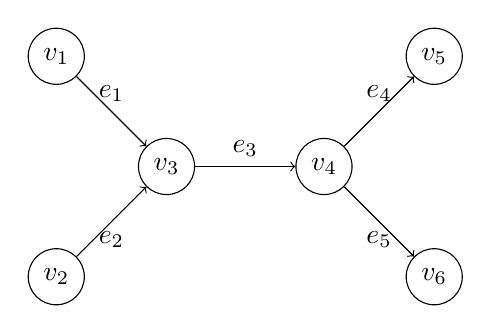
\begin{tikzpicture}
            % vertices
            \node[shape=circle,draw=black] (v1) at (-2.4,1.4) {$v_1$};
            \node[shape=circle,draw=black] (v5) at (2.4,1.4) {$v_5$};
            \node[shape=circle,draw=black] (v3) at (-1,0) {$v_3$};
            \node[shape=circle,draw=black] (v4) at (1,0) {$v_4$};
            \node[shape=circle,draw=black] (v2) at (-2.4,-1.4) {$v_2$};
            \node[shape=circle,draw=black] (v6) at (2.4,-1.4) {$v_6$};
            
            % edges
            \path [->](v1) edge node[above] {$e_1$} (v3);
            \path [->](v2) edge node[below] {$e_2$} (v3);
            \path [->](v3) edge node[above] {$e_3$} (v4);
            \path [->](v4) edge node[above] {$e_4$} (v5);
            \path [->](v4) edge node[below] {$e_5$} (v6);
        \end{tikzpicture}
    \end{center}
    \caption{The metric graph $\Gamma$ defined by equation \cref{NumericalExperimentGraph} plotted.}
    \label{fig7}
\end{figure}
As we can see, the vertices $v_1$, $v_2$, $v_5$ and $v_6$ are the exterior vertices, i.e. $\mathcal{V}_{\mathcal{D}} = \left\{v_1, v_2, v_5, v_6 \right\}$, and the vertices $v_3$ and $v_4$ are the interior vertices, i.e. $\mathcal{V}_{\mathcal{K}} = \left\{v_3, v_4 \right \}$, of the graph $\Gamma$. \\
As an approximation problem, we consider the set of drift-diffusion equations defined by \cref{Drift-Diffusion-equation} on all edges $e \in \mathcal{E}$ of the graph $\Gamma = \left(\mathcal{V}, \mathcal{E} \right)$, which is defined by \cref{NumericalExperimentGraph}, under the initial and vertex conditions given by \cref{eq:Kirchhoff_Neumann_condition}, \cref{continuous on vertices}, \cref{eq:Dirichlet_conditions} and \cref{eq:initial_conditions}. Furthermore we have the following assumptions:
\begin{assumption} \label{graph_assumptions} 
    \ \\[-1.5\baselineskip]
    \begin{enumerate}
        \item The observation time ends at $T = 10$ and the graph $\Gamma$ is equilateral (see \cref{metric graph equilateral}) with $\ell = 1$. 
        \item Let $\varepsilon = 0.01$ in \cref{Drift-Diffusion-equation}.
        \item The mobility in \cref{Drift-Diffusion-equation} is given by $f \left( \rho_e(t,x) \right) = \rho_e \left(t,x\right)\left(1-\rho_e \left(t,x\right)\right)$.
        \item $\partial_x V_e \left(t,x\right) = 1$ for all $\left(t,x\right) \in \left(0, 10\right) \times \left[0,1\right]$ holds in \cref{Drift-Diffusion-equation} for the potential $V_e$ of each edge $e \in \mathcal{E}$. 
        \item On the exterior vertices $\mathcal{V}_{\mathcal{D}}$, we have for the flux vertex conditions, \cref{eq:Dirichlet_conditions}, constant influx and outflux rates which are specified for $v_1$ by $\alpha_{v_1}\left(t\right) = 0.9$ and $\beta_{v_1}\left(t\right) = 0$, for $v_2$ by $\alpha_{v_2}\left(t\right) = 0.3$ and $\beta_{v_2}\left(t\right) = 0$, for $v_5$ by $\alpha_{v_5}\left(t\right) = 0$ and $\beta_{v_5}\left(t\right) = 0.8$ and for $v_6$ by $\alpha_{v_6}\left(t\right) = 0$ and $\beta_{v_6}\left(t\right) = 0.1$.
        \item The initial conditions are $\rho_e\left(0,x\right) = 0$ for all $x \in \left[0, \ell_e\right]$ for each edge $e \in \mathcal{E}$. 
    \end{enumerate}
\end{assumption}

In the following, we specify the neural networks and their topology that we use to approximate the solution $\rho_{\theta_e}$ of \cref{Drift-Diffusion-equation} on an individual edge $e \in \mathcal{E}$ under the given initial and vertex conditions in the numerical experiments. Of course, we have an infinite freedom of choice, the only constraints being the dimension of the input $\left(t, x\right) \in \mathbb{R}^2$, the dimension of the output $\rho_{\theta_e}\left(t, x\right) \in \mathbb{R}$ and the differentiability of the corresponding neural network up to order two (due to $\partial_{xx} \rho_{\theta_e}$ appearing in \cref{Drift-Diffusion-equation}). We now introduce three different types of neural networks for the approximation of $\rho_e \colon \left(0, T\right) \times \left[0, \ell_e\right] \to \mathbb{R}$, which we use in the numerical experiments. \\
Since we have to find an approximation $\rho_{\theta_e}$ for each edge $e \in \mathcal{E}$ and since these approximations $\left\{ \rho_{\theta_e} \right\}_{e \in \mathcal{E}}$ are individually included in the cost function $\Phi_{\theta}$, it is quite evident to use one single neural network for the approximation of the solution of \cref{Drift-Diffusion-equation} on one individual edge $e$. This results in the fact that we use as many neural networks as we have edges of the graph $\Gamma$. In this case, $\theta_e$ describes the trainable parameters of a single neural network and $\theta$ is the union of the trainable parameters of all neural networks. Thus, during the learning phase, all trainable parameters $\theta$ are modified when the cost function $\Phi_{\theta}$ is minimized, and therefore consider the used optimization methods $\theta$ as the optimization variable. Using one neural network for the approximation of the solution on one edge offers the possibility to select individual hyperparameters like the topology or the activation functions for the different neural networks. One can use a deep neural network for an edge for which the solution can have a complex structure, while a shallow neural network can be used on the edges with relatively simple and smooth solutions. In this work, however, we will not cover such a case due to the effort of finding the best hyperparameters for each neural network, we just use the same type of neural network with the same topology for the approximation of $\rho_e$ each edge $e \in \mathcal{E}$. \\

We pursue this idea of using a single neural network to approximate $\rho_e$ on a single edge $e \in \mathcal{E}$. The easiest choice is to use a feed-forward neural network with $L$-layers for each edge $e \in \mathcal{E}$, which we denote by $\operatorname{fnn}_{\theta_e}$ and is defined by 
\begin{equation} 
    \label{one_for_each}
    \begin{gathered}
        \operatorname{fnn}_{\theta_e} \colon \mathbb{R}^2 \to \mathbb{R}, \\
        \\
        \operatorname{fnn}_{\theta_e}\left(t, x\right) = \sigma_L\left(W^L_e \sigma_{L-1}\left(W^{L-1}_e\sigma_{L-2}\left(\cdots \sigma_{1}\left(W^{1}_e x^0 +b^1_e\right) \cdots\right) + b^{L-1}_e\right) + b^{L}_e\right),
    \end{gathered} 
\end{equation} 
where $x^0 = \left(t, x\right)^{\mathrm{T}} \in \left(0, T\right) \times \left[0, \ell_e\right] \subset \mathbb{R}^2$ and $\theta_e = \left\{ \left\{ W^l_e \right\}_{l = 1, \ldots, L}, \left\{ b^l_e \right\}_{l = 1, \ldots, L} \right\}$ with $W^l_e \in \mathbb{R}^{n_l \times n_{l-1}}$ and $b^l_e \in \mathbb{R}^{n_l}$, where $n_0 = 2$ and $n_L = 1$. The total set of all trainable parameters for the resulting $PINN$ approach is therefore $\theta = \bigcup_{e \in \mathcal{E}} \ \theta_e$. Feed-forward neural networks have already been used in various $PINN$ setups, so this choice can be considered as reasonable. \\

Of course, other neural networks with one-dimensional output can also be used, such as the one described by the following architecture and the following forward propagation 
\begin{equation} 
    \label{Resnet1}
    \begin{gathered}
        \operatorname{R}_{\theta_e} \colon \mathbb{R}^2 \to \mathbb{R}, \\
        \\
        \operatorname{R}_{\theta_e}\left(x^0\right) = \frac{1}{2} {x^0}^{\mathrm{T}} A_e x^0 + {x^{L}}^{\mathrm{T}} w_e + c^{\mathrm{T}}_e x^0,
    \end{gathered} 
\end{equation} 
with
\begin{equation}
    \label{Resnet2} 
    \begin{gathered}
        x^1 = \sigma_1\left(W^1_e x^{0} + b^1_e\right) \in \mathbb{R}^m, \\
        \\
        x^l = x^{l-1} + h \, \sigma_l\left(W^l_e x^{l-1} + b^l_e\right) \in \mathbb{R}^m \quad \text{for} \quad l = 2, \ldots, L, 
    \end{gathered} 
\end{equation} 
where $h > 0$ is called stepsize and is a hyperparameter, $x^0 = \left(t, x\right)^{\mathrm{T}} \in \left(0, T\right) \times \left[0, \ell_e\right]$, $W^1_e \in \mathbb{R}^{m \times 2}$ and $W^l_e \in \mathbb{R}^{m \times m}$ for $l = 2, \ldots, L$, $b^l_e \in \mathbb{R}^{m}$ for $l = 1, \ldots, L$ and $A_e \in \mathbb{R}^{2 \times 2}$, $w_e \in \mathbb{R}^m$, $c_e \in \mathbb{R}^2$ are also trainable parameters, i.e. \\
$\theta_e = \left\{ \left\{ W^l_e \right\}_{l = 1, \ldots, L}, \left\{ b^l_e \right\}_{l = 1, \ldots, L}, A_e, w_e, c_e \right\}$ and $\theta = \bigcup_{e \in \mathcal{E}} \ \theta_e$. The idea of using this type of neural network originates from \cite{RuthottoOsherLiNurbekyanFung2020}, in which high-dimensional mean field games and mean field control models are approximately solved by combining Lagrangian and Eulerian viewpoints and by using a tailored neural network parameterization for the potential of the solution, which can be understood as a density, to avoid any spatial discretisation. The neural network given by the forward propagation in \cref{Resnet2} is also called residual network and abbreviated with $ResNet$, \cite{HeZhangRenSun:2015}. We refer to it only as $ResNet$ to avoid confusion with the residual network of a $PINN$. $ResNet$s have been successful in a wide range of machine learning tasks and have been found to be trainable even for many layers. By interpreting \cref{Resnet2} as a forward Euler discretization of an initial value problem, the continuous limit of a $ResNet$ is amenable to mathematical analysis, \cite[p.~6]{RuthottoOsherLiNurbekyanFung2020}. \\

 It is also possible to use just one single $FNN$ with $L$ layers for the approximation of the solution of \cref{Drift-Diffusion-equation} under the given initial and vertex conditions on all edges of the graph $\Gamma$. This means that this single $FNN$ returns for a point $\left(t,x\right) \in \mathbb{R}^2$ the values $\left\{ \rho_{\theta_{e_i}}\left(t, x\right) \right\}_{i = 1, \ldots, E}$ for all edges $\mathcal{E} = \left\{ e_i \right\}_{i = 1, \ldots, E}$, where $E = \abs{\mathcal{E}}$. This is achieved by choosing the number of neurons in the output layer equal to the number of edges of the graph, i.e. $n_L = E$. We define this neural network as follows
\begin{equation} 
    \label{one_for_all}
    \begin{gathered}
        \operatorname{FNN}_{\theta} \colon \mathbb{R}^2 \to \mathbb{R}^E \\
        \\
        \operatorname{FNN}_{\theta}\left(t, x\right) = \sigma_L\left(W^L \sigma_{L-1}\left(W^{L-1}\sigma_{L-2}\left(\cdots \sigma_{1}\left(W^{1}x^0 +b^1\right) \cdots\right) + b^{L-1}\right) + b^{L}\right) \in \mathbb{R}^E, 
    \end{gathered} 
\end{equation} 
where $x^0 = \left(t, x\right)^{\mathrm{T}} \in \left(0, T\right) \times \left[0, \ell_e\right] \subset \mathbb{R}^2$ and $\theta = \left\{ \left\{ W^l \right\}_{l = 1, \ldots, L}, \left\{ b^l \right\}_{l = 1, \ldots, L} \right\}$ with $W^l \in \mathbb{R}^{n_l \times n_{l-1}}$ and $b^l \in \mathbb{R}^{n_l}$, where $n_0 = 2$ and $n_L = E$. The individual approximations are given by 
\begin{equation*}
    \rho_{\theta_{e_i}}\left(t, x\right) = \left[ \operatorname{FNN}_{\theta}\left(t, x\right) \right]_i \in \mathbb{R},
\end{equation*}
i.e. the $i$-th entry of the networks output $\operatorname{FNN}_{\theta}\left(t, x\right) \in \mathbb{R}^E$ is the approximation of the solution on the $i$-th edge. We see that in this case $\theta$ consists only of the weights and biases of this single neural network, as indicated by the index $\theta$ in $\operatorname{FNN}_{\theta}$. \\
The use of a single neural network is motivated by the hope that the neurons in the hidden layers will learn the structure of the entire graph and the resulting communication of the edges via the vertices, i.e. that all interactions within the graph are taken into account by the neurons after the learning phase. Furthermore, we hope that the computational cost is reduced, since only the weights and biases of this single network need to be trained, provided the depth and width of the neural network $\operatorname{FNN}_{\theta}$ are not too large. The fact that $\operatorname{FNN}_{\theta}\left(t, x\right)$ generates the output for all edges at the same time is also an advantage, as in an implementation only the execution of one network is necessary instead of several. However, we point out that this approach of using just one single neural network only makes sense if the graph is equilateral (as we have assumed above for the metric graph $\Gamma$, see \cref{graph_assumptions}), because then the same collocation points $X_e = \{ \left( t_e^i, x_e^i \right)\}_{i=1}^{n_e}$ and $X_{e,0} = \{x_{e,0}^i\}_{i=1}^{n_0}$ can be used for the misfit terms given by \cref{misfit:residual} and \cref{misfit:initial} for all edges $e \in \mathcal{E}$. \\

With the cost function defined by \cref{eq:loss:1} and the three different types of neural networks defined above, we perform numerical experiments in which these neural networks are trained using $\Phi_{\theta}$ for the approximation problem, which is given by the set of drift-diffusion equations given by \cref{Drift-Diffusion-equation} on the metric graph defined by \cref{NumericalExperimentGraph} under the initial and vertex conditions and the given \cref{graph_assumptions}. To compare the Performance of the neural networks we use as ground truth values generated by the $FVM$ described in \cref{ch2} with the time discretization $N_t = 5000$ and the space discretization $N_e = 1001$ on each edge $e \in \mathcal{E}$ as a benchmark solution and we measure in the resulting three numerical experiments the difference between them and the values of the trained neural networks at the same grid points given by the discretization. For the first numerical experiment, we use the $FNN$ described by \cref{one_for_each} with $3$ layers, where we chose $n_0 = 2$, $n_1, n_2 = 10$ and $n_3 = 1$. The hyperbolic tangent function defined by \cref{TanH} is used as activation function for all hidden layers as well as for the output layer. For the second numerical experiment, we used the $ResNet$ described by \cref{Resnet1}, where $x^L$ is computed by \cref{Resnet2} using $L = 3$ layers with $m = 12$. The stepsize is $h=1$ and the hyperbolic tangent function defined by \cref{TanH} was used as activation function in all layers. For the third and final numerical experiment, we use the $FNN$ described by \cref{one_for_all} with $4$ layers, where we chose $n_0 = 2$, $n_1, n_2, n_3 = 20$ and $n_4 = 5$. Also here, the hyperbolic tangent function defined by \cref{TanH} is used as activation function for all hidden layers as well as for the output layer. \\
As already mentioned, the numerical experiments are implemented with \lstinline!Python 3.8.8! and were run on a Lenovo ThinkPad L490, 64 bit Windows system, 1.8 Ghz Intel Core i7-8565U and 32 GB RAM. \\
All collocation points are randomly generated using \lstinline!tf.random.uniform!, which is provided by the package \lstinline!Tensorflow!, see \cite{TensorFlow}, and uses an normal distribution. Further we set \lstinline!dtype = 'float64'!. As time-space collocation points $X_e$ for \cref{misfit:residual} we use $n_e = 4000$ randomly selected points $\left\{ \left( t_e^i, x_e^i \right) \right\}_{i=1}^{n_e} \subset \left( 0, T \right) \times \left[0, \ell_e\right]$. As space collocation points $X_{e,0}$ for \cref{misfit:initial} we use $n_0 = 1000$ randomly selected points $ \left\{ x_{e,0}^i \right\}_{i=1}^{n_0} \subset \left[0, \ell_e\right]$. For \cref{misfit:Kirchhoff}, \cref{misfit:Dirichlet} and \cref{misfit:continuity} we use $n_b = 1000$ randomly chosen points $\left\{ t_{0,b}^i \right\}_{i=1}^{n_b} \subset \left( 0,T \right)$ as time snapshots $X_{0,b}$ for origin vertices, i.e. $v = 0$, and $n_b = 1000$ randomly chosen points as time snapshots $X_{1,b}$ for terminal vertices, i.e. $v = 1$ (we recall that the graph $\Gamma$ is equilateral). \\
For the minimization of the cost function $\Phi_{\theta}$, we first use a variant of the gradient descent method, in which the direction is given by the Adam optimizer from the module \lstinline!Keras!, see \cite{Chollet:2015}, which belongs to the package \lstinline!Tensorflow!, see \cite{TensorFlow}. We change for the different types of neural networks the input parameter \lstinline!learning_rate!, which obviously specifies the learning rate of the method, and leave all other input parameters of the Adam optimizer by default. This method stops after $2000$ iterations. After that, we use the L-BFGS-B optimizer from the package \lstinline!SciPy!, see \cite{SciPy:2020}, and we set for all networks as parameters in the options \lstinline!maxiter = 50000! which specifies the maximum number of iterations, \lstinline!maxfun = 500000! which specifies the maximum number of function evaluations, \lstinline!maxcor = 50! which specifies the maximum number of stored variable metric corrections used in the L-BFGS approximation of the Hessian of the cost function $\Phi_{\theta}$, \lstinline!maxls = 50! which specifies the maximum number of line search steps per iteration and \lstinline!ftol = 1.0*np.finfo(float).eps! which specifies a parameter in a stopping criterion that aborts the method if the values of the cost function $\Phi_{\theta}$ between two iterates are too small. \\
We note that, as mentioned in \cref{ch1:sec4}, all derivatives of the surrogate models with respect to the input, i.e. the values $\partial_x \rho_{\theta_e}  \left( t, x \right)$, $\partial_t \rho_{\theta_e}  \left( t, x \right)$, $\partial_{xx} \rho_{\theta_e}  \left( t, x \right)$ for $(t, x) \in $ are computed using $AD$, which is provided by \lstinline!Tensorflow! via the method \lstinline!tf.GradientTape!. \\
The results of the numerical experiments are summarised in \cref{tab:neural networks}. The first row specifies the used neural networks. The second row contains the values of the cost function $\Phi_{\theta} \left( \operatorname{X} \right)$ evaluated at the union of the collocation points, with which the neuronal networks have completed the learning phase. The third row contains the $L^2$-error, which results from the $L^2$-norm of the difference between the values generated by the trained neural network and the values generated by the $FVM$ on the same point grid. For each edge, the point grid consists of $5 \cdot 10^{6}$ equidistantly chosen points $(t, x) \in \left(0, 10\right) \times \left[0,1\right]$. Thus, the $L^2$-error is measured over $25 \cdot 10^{6}$ points. The learning phase ended for all neural networks after the L-BFGS-B optimizer reached its maximum number of iterations, which is $5 \cdot 10^{4}$. \\

\begin{table}[H]
    \resizebox{\textwidth}{!}{
        \begin{tabular}{l l l l }
            \toprule
            Neural Network & $\operatorname{fnn}_{\theta_e}$ & $\operatorname{R}_{\theta_e}$ & $\operatorname{FNN}_{\theta}$  \\ 
            \midrule
            $\Phi_{\theta} \left( \operatorname{X} \right)$ & $3.63 \cdot 10^{-4}$ & $3.05 \cdot 10^{-2}$ & $4.46 \cdot 10^{-4}$  \\
            \midrule
            $L^2$-Error & $275.64$ & $1530.23$ & $430.45$ \\ 
            \bottomrule
        \end{tabular}
    }
    \caption{The values of the cost function $\Phi_{\theta} \left( \operatorname{X} \right)$ and the $L^2$-Error with respect to the values generated by the $FVM$ method of the three different neural networks after the learning phase.}
    \label{tab:neural networks}
\end{table}

The values in \cref{tab:neural networks} show that using the $FNN$ $\operatorname{fnn}_{\theta_e}$ for each edge $e \in \mathcal{E}$ of the graph $\Gamma$ provides the best approximation of those tested, as both the cost function value $\Phi_{\theta} \left( \operatorname{X} \right)$ and the $L^2$-error are the lowest. The $PINN$ approach using the $ResNet$ $\operatorname{R}_{\theta_e}$ for each edge $e \in \mathcal{E}$ performed the worst. Using the single $FNN$ $\operatorname{FNN}_{\theta}$ for all edges gives appropriate results but, since all methods were aborted by the same stopping criterion (maximum number of iterations reached), it shows that the $FNN$ $\operatorname{fnn}_{\theta_e}$ is the superior choice as it was better trained with the same number of iterations. We note that these results only allow conclusions to be drawn for these specific neural networks with this specific topology and provide almost no indication of the general ability of a type of neural network to be used in this approach.  \\
Although the error of the neural network $FNN$ $\operatorname{fnn}_{\theta_e}$ seems very significant, one must of course take into account that it was evaluated over $25 \cdot 10^{6}$ points. This results in an average error of $1.10 \cdot 10^{-5}$ for each point. Thus, the use of this network $\operatorname{fnn}_{\theta_e}$ in the $PINN$ approach defined by the cost function $\Phi_{\theta}$ given by \cref{eq:loss:1} seems to be a reasonable choice to use for approximating the solutions of the drift-diffusion equations given by \cref{Drift-Diffusion-equation} on the edges of the metric graph defined by \cref{NumericalExperimentGraph} under the \cref{graph_assumptions}. The following figures, in which the approximation values of the neural network $\operatorname{fnn}_{\theta_e}$ on one edge are compared to the approximation values of the $FVM$ on the same edge, illustrate that this $PINN$ approach using this $FNN$ $\operatorname{fnn}_{\theta_e}$ for each edge produces a smooth approximate solution and thus provides an alternative to the $FVM$. \\

\begin{figure}[H]
    \begin{center}
        \begin{subfigure}[b]{0.4\textwidth}
            \begin{center}
                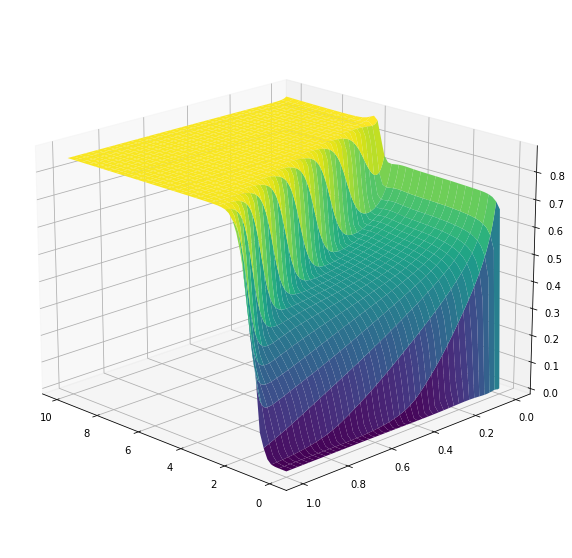
\includegraphics[scale=0.35]{img/Kante1.png}
            \end{center}
            \caption{$\operatorname{fnn}_{\theta_{e_1}}$}
        \end{subfigure} \hspace{15mm}
        \begin{subfigure}[b]{0.4\textwidth}
            \begin{center}
                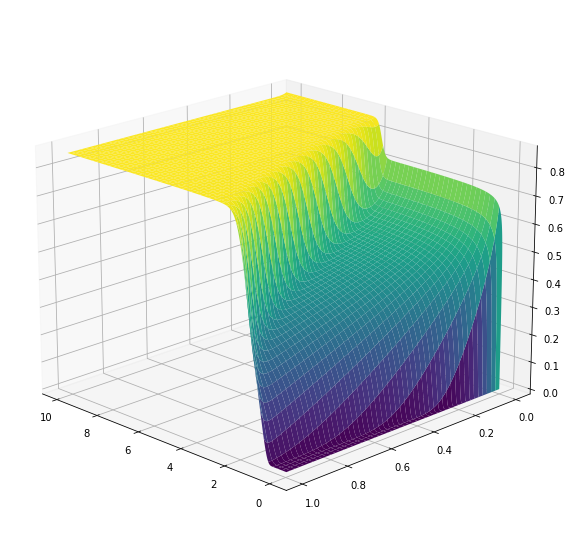
\includegraphics[scale=0.35]{img/FVM1.png}
            \end{center}
            \caption{$FVM$ on $e_1$}
        \end{subfigure}
    \end{center}
\end{figure}
\begin{figure}[H]
    \begin{center}
        \begin{subfigure}[b]{0.4\textwidth}
            \begin{center}
                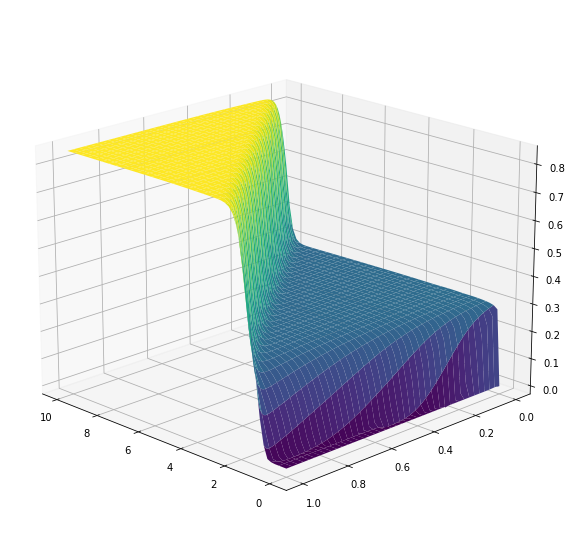
\includegraphics[scale=0.35]{img/Kante2.png}
            \end{center}
            \caption{$\operatorname{fnn}_{\theta_{e_2}}$}
        \end{subfigure} \hspace{15mm}
        \begin{subfigure}[b]{0.4\textwidth}
            \begin{center}
                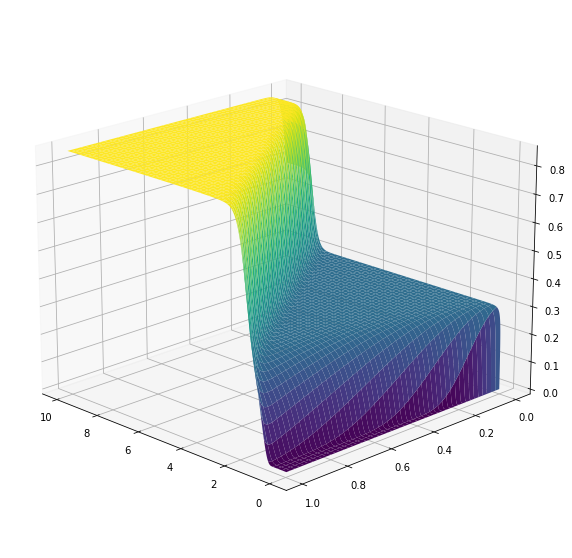
\includegraphics[scale=0.35]{img/FVM2.png}
            \end{center}
            \caption{$FVM$ on $e_2$}
        \end{subfigure}
    \end{center}
\end{figure}
\begin{figure}[H]
    \begin{center}
        \begin{subfigure}[b]{0.4\textwidth}
            \begin{center}
                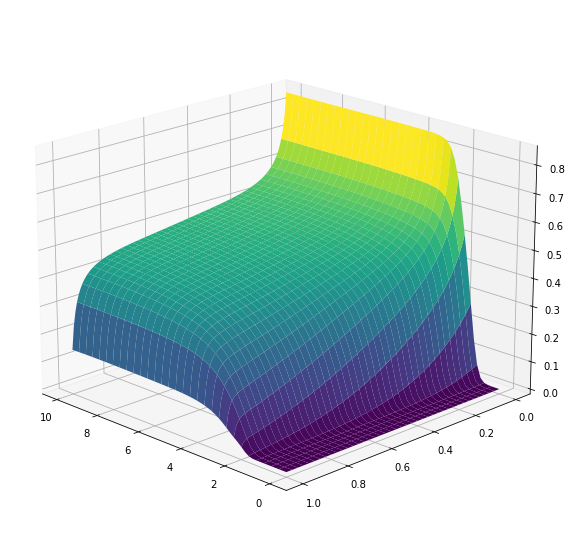
\includegraphics[scale=0.35]{img/Kante3.png}
            \end{center}
            \caption{$\operatorname{fnn}_{\theta_{e_3}}$}
        \end{subfigure} \hspace{15mm}
        \begin{subfigure}[b]{0.4\textwidth}
            \begin{center}
                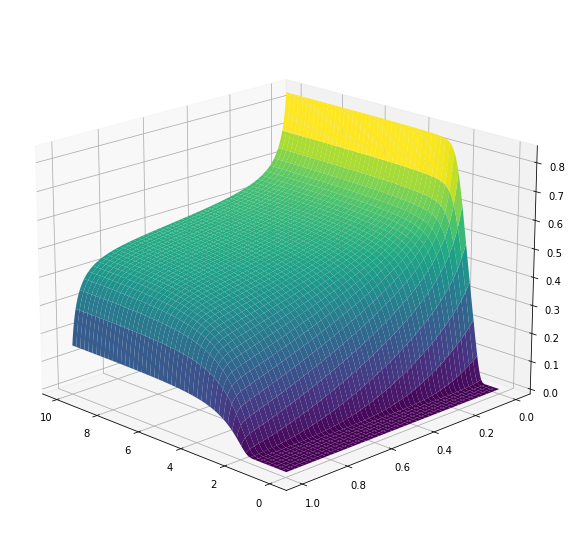
\includegraphics[scale=0.35]{img/FVM3.png}
            \end{center}
            \caption{$FVM$ on $e_3$}
        \end{subfigure}
    \end{center}
\end{figure}
\begin{figure}[H]
    \begin{center}
        \begin{subfigure}[b]{0.4\textwidth}
            \begin{center}
                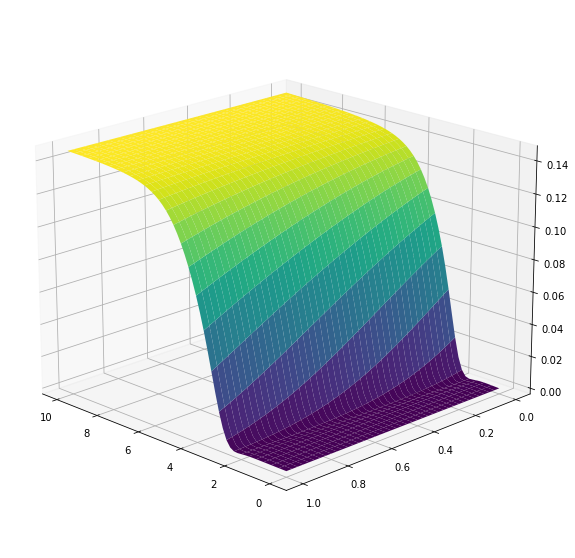
\includegraphics[scale=0.35]{img/Kante4.png}
            \end{center}
            \caption{$\operatorname{fnn}_{\theta_{e_4}}$}
        \end{subfigure} \hspace{15mm}
        \begin{subfigure}[b]{0.4\textwidth}
            \begin{center}
                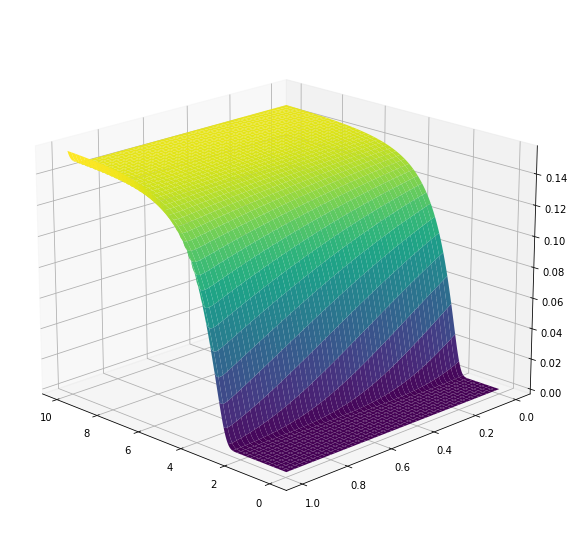
\includegraphics[scale=0.35]{img/FVM4.png}
            \end{center}
            \caption{$FVM$ on $e_4$}
        \end{subfigure}
    \end{center}
\end{figure}
\begin{figure}[H]
    \begin{center}
        \begin{subfigure}[b]{0.4\textwidth}
            \begin{center}
                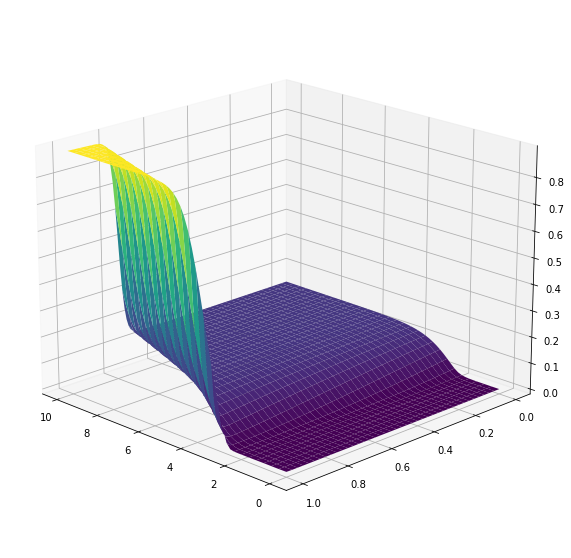
\includegraphics[scale=0.35]{img/Kante5.png}
            \end{center}
            \caption{$\operatorname{fnn}_{\theta_{e_5}}$}
        \end{subfigure} \hspace{15mm}
        \begin{subfigure}[b]{0.4\textwidth}
            \begin{center}
                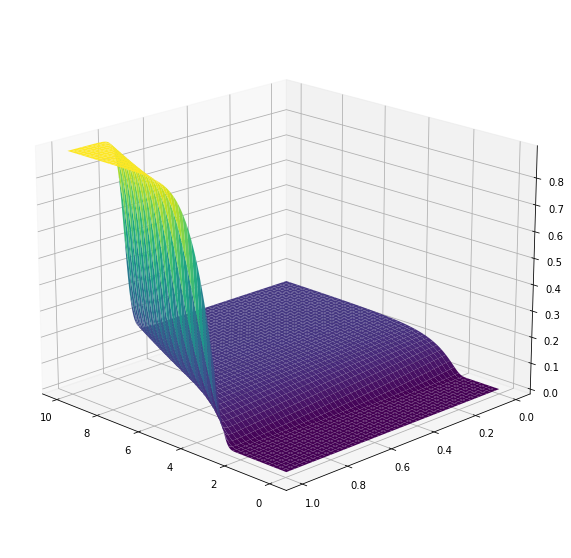
\includegraphics[scale=0.35]{img/FVM5.png}
            \end{center}
            \caption{$FVM$ on $e_5$}
        \end{subfigure}
    \end{center}
\end{figure}

In conclusion, it has been shown that the solutions of the drift-diffusion equations given by \cref{Drift-Diffusion-equation} on the edges $e \in \mathcal{E}$ of a metric graph $\Gamma = \left(\mathcal{V}, \mathcal{E} \right)$ can be approximated with this $PINN$ approach. The construction of the cost function $\Phi_{\theta}$ follows the usual principle for this purpose and by minimising it, a appropriately selected neural network can be trained. The comparison of the measured $L^2$-Error with the $FVM$ at the same grid points has shown that the choice of a suitable neural network and also the choice whether one uses one neural network for all edges or one neural network for each edge can have an effect on the approximation quality. Finally, we note that of course other $PINN$ approaches can be designed for this or similar problems, in which the cost function can have a different form or the structure of the graph can be exploited differently. Also, the selection of the used neural network can be improved by $NAS$ methods and the topology of the neural network can be refined by hyperparameter optimization. \\

%fnn: Experiment 1: Loss $3.63346069e-04$ , STOP: TOTAL NO. of ITERATIONS REACHED LIMIT, L2 Error 275.6428860459677, Sup Error 0.5521403415528678
%Resnet: Loss  $3.05133775e-02$   4212.47, STOP: TOTAL NO. of ITERATIONS REACHED LIMIT, L2 Error 1530.2266754494092, Sup Error 0.8705551259854093
% FNN: $4.46322321e-04$  5247.55, STOP: TOTAL NO. of ITERATIONS REACHED LIMIT, L2 Error 430.4514416907528, Sup Error 0.7684574683811376
